\documentclass{../template/tp}
\usepackage[utf8x]{inputenc}

\usepackage[frenchb]{babel}
\usepackage[T1]{fontenc}

\usepackage{graphicx}
\usepackage{amssymb}
\usepackage{amsmath}
\usepackage{wasysym} %smiley
\usepackage{hyperref}% hyperliens
\usepackage{tikz}
\usetikzlibrary{babel,positioning,calc}
\usepackage[]{circuitikz}
\usepackage{textcomp}
% \usepackage{minted}
\usepackage[long]{datetime}
\usepackage{gensymb} % \ohm, celsius
\usepackage{framed}
\usepackage{pdfpages}
\usepackage{todo}
\usepackage{paralist}
\usepackage{multicol}

\usepackage{mathastext} % math as standfard text : units are respecting typography conventions.
\usepackage{fancyhdr} %en-tête
\usepackage{qrcode}
\usepackage{pgfplots} %for latex grid

\langexam{frenchb}

\correction{false}
%\correction{true}

\author{The Fantastic Four} %<3


%% fancy header & foot
\pagestyle{fancy}
\lhead{[ELEC-H-301] Électronique appliquée\\ LABO \no 1 : Filtrage\ifthenelse{\boolean{corrige}}{~-- corrigé}{}}
\rhead{v1.0.4\\ page \thepage}
\cfoot{}
%%

\pdfinfo{
/Author (Raoul Sommeillier, ULB -- BEAMS)
/Title (LABO 1 ELEC-H-301, Filtrage)
/ModDate (D:\pdfdate)
}

\hypersetup{
pdftitle={LABO 1 [ELEC-H-301] Électronique appliquée: Filtrage},
pdfauthor={Raoul Sommeillier, ©2017 ULB - BEAMS  },
pdfsubject={Filtrage}
}

%\date{\vspace{-1cm}\mydate\today}
%\title{\vspace{-2cm} Labo \no 6\\ Électronique appliquée [ELEC-H-301]\\Réalisation d'un ampli à transistor\ifthenelse{\boolean{corrige}}{~\\Corrigé}{}}

%\author{\vspace{-1cm}}%\textsc{Yannick Allard}}

\setlength{\parskip}{0.5cm plus4mm minus3mm} %espacement entre §
\setlength{\parindent}{0pt}


\begin{document}

\tptitle{}{Séance 1~: Filtrage}

\section{But de la manipulation}

Les compétences devant être développées par l'étudiant à la fin de cette séance sont en particulier:
\begin{itemize}
	\item vous familiariser avec les instruments de mesure qui seront utilisés dans les laboratoires ultérieurs: générateur de fonctions, multimètre et oscilloscope ;
	\item étudier une des fonctions de base en électronique : le filtrage (en particulier les circuits RC et RLC) ;
	\item utiliser les outils mathématiques de l'analyse fréquentielle, qui conviennent particulièrement bien pour étudier les
circuits précédents.
\end{itemize}

\section{Pré-requis}
L'ensemble du cours d'électricité BA2, partie « théorie des circuits » est supposé connu avant ce laboratoire.\\
On y utilisera en particulier les notions suivantes :
\begin{itemize}
\item masse et terre ; % (syllabus BA2 §1.5) ;
\item équivalents de Thévenin et de Norton, impédances d'entrée et de sortie ; %(syll. BA2 §4) ;
\item analyse fréquentielle d'un circuit réactif : valeur efficace, plan de Bode, rapports de tension en
décibels, rapports de fréquence en décades et octaves, phaseurs, fonction de transfert et réponse indicielle d'un
circuit linéaire, fréquence de coupure, etc. ; %syll. BA2 §7 et 8)
\end{itemize}
On vous demande également de lire:
\begin{itemize}
\item les annexes expliquant le principe de fonctionnement et les fonctionnalités des appareils de mesure du laboratoire;
\item le document intitulé « fonctions de transfert et plan de Bode », qui couvre la même matière que le syllabus BA2.
%§8.
\end{itemize}

\section{Matériel}
En plus du matériel classique de laboratoire (multimètre, oscilloscope, générateur de fonction, câbles, etc.), cette séance nécessite les composants suivants:
\begin{itemize}
\item Résistances : une de $390\Omega$ et une de $10k\Omega$
\item Condensateurs : un de $10nF$ et un de $33nF$
\item Inductance : une de $8,2mH$
\end{itemize}

\newpage
\section{Préliminaire théorique} %{\normalsize{(1 point)}}}
Avant d'entrer au laboratoire, il est encore conseillé de réaliser les prédéterminations des §6.2, §6.3.2 et §6.4.2 de cet énoncé.

\section{Objectifs}
A la fin de ce laboratoire, vous devez être capable :
\begin{itemize}
\item d'expliquer le principe de fonctionnement des différents appareils utilisés,
\item d'utiliser les principales fonctionnalités de ces appareils,
\item d'expliquer les notions de masse, terre et borne « common »,
\item de relever (mesure) la fonction de transfert d'un circuit réel,
\item de tracer une fonction de transfert dans un plan de Bode à partir de son expression mathématique (théorie) ou de
mesures (pratique),
\item d'utiliser les phaseurs et les impédances complexes.
\end{itemize}



\section{Manipulation}
\subsection{Remarques préliminaires à propos du câblage}
Afin de simplifier la vérification du câblage, d'éviter des erreurs et de limiter l'émission/réception de parasites, on
respectera les règles suivantes :
\begin{itemize}
\item utilisez intelligemment les couleurs : des fils de couleurs différentes vous sont fournis, ils vous permettent de
repérer plus facilement les différents types de signaux une fois le montage achevé. En particulier :
\item le noir est réservé à la masse du circuit ;
\item ne connectez jamais 2 fils de couleurs différentes au même noeud.
\item disposez les appareils et autres éléments dans l'ordre où ils apparaissent sur le schéma électrique.
\item évitez les distances inutilement longues.
\item évitez les croisements (par exemple ne placez pas le voltmètre mesurant la tension de sortie près de l'entrée du
montage et le générateur d'entrée près de la sortie).
\end{itemize}
Un signal électrique implique la circulation d'un courant, donc un conducteur aller et un conducteur retour. Il y a lieu
de disposer physiquement ces deux conducteurs aussi près l'un de l'autre que possible, pour éviter de créer une boucle
risquant de capter ou de générer un signal parasite sous forme d'un champ magnétique (cfr cours chap. 3).

\subsection{Lecture préliminaire}

En annexe de cet énoncé, nous avons écrit un document décrivant le générateur de fonction, le multimètre,
l'oscilloscope et le protoboard que vous utiliserez lors de vos laboratoires d'électronique.
On vous demande de les lire avant d'arriver au labo.\\
En particulier,
\begin{itemize}
\item pour chacun des appareils, vous devrez être capable de donner le schéma équivalent de son entrée ou de sa
sortie;
\item pour les deux appareils de mesure, vous devrez pouvoir :
\item expliquer la différence entre la mesure DC et la mesure AC,
\item avoir une idée de leur bande passante,
\item savoir si ils peuvent faire des mesures différentielles.
\end{itemize}
Au besoin, vous pouvez commencer la manipulation en vérifiant par l'expérience ce qui est décrit dans ces
documents.
\subsection{Le circuit RC passe-haut}
\subsubsection{Introduction}
Le circuit RC passe-haut peut être vu comme un quadripôle :
\begin{center}
\begin{circuitikz} \draw
(0,0)   node[ground]{}
		to[american voltage source, v=$V_{in}$, invert] 	(0,3)
		to[C, l=$C$]									(3,3)
		(3,0) to[R, l=$R$, v=$V_{out}$] (3,3)
		(3,0)--(0,0)
;
\end{circuitikz}
\end{center}
Pour établir sa fonction de transfert, le plus simple est de remarquer que le circuit RC est un diviseur impédant (c'est à dire la généralisation du diviseur résistif à n'importe quel type d'impédance). On peut donc écrire :
$$\underline{V}_{out}(p)=\frac{Z_R(p)}{Z_R(p)+Z_C(p)}\underline{V}_{in}(p)=\frac{Z_R(p)}{Z_{tot}(p)}\underline{V}_{in}(p)$$

\subsubsection{Prédéterminations : tracé asymptotique de la réponse fréquentielle}
\textbf{Approche mathématique}\\
Remarque : nous avons écrit un document détaillant cette méthode : « Fonctions de transfert et plan de Bode »
\begin{itemize}
\item Établissez l'expression de la fonction de transfert du circuit $H(p)=\frac{\underline{V}_{out}(p)}{\underline{V}_{in}(p)}$
\item Calculez les pôles et zéros de la fonction de transfert.
\item Déduisez, de la fonction de transfert, la réponse fréquentielle du circuit $H(j\omega)=\frac{\underline{V}_{out}(j\omega)}{\underline{V}_{in}(j\omega)}$
\item Tracez l'approximation asymptotique de la réponse fréquentielle dans un plan de Bode (donné en annexe).
\end{itemize}

\textbf{Approche intuitive}
Nous pouvons aussi déduire le comportement asymptotique de la réponse fréquentielle par un raisonnement sur les impédances, en se rappelant que :
$H(j\omega)=\frac{Z_R(j\omega)}{Z_{tot}(j\omega)}$

\Question
{
Répondez aux questions suivantes pour chacun des cas $\omega \Rightarrow 0$ et  $\omega \Rightarrow \infty$:
\begin{itemize}
\item $Z_{tot}$ est la somme de deux impédances, laquelle des deux peut-on négliger ?
\item Déduisez-en une expression approchée de la réponse fréquentielle à la pulsation considérée.
\item Quelle relation pouvez-vous écrire entre les modules de $Z_R$ et $Z_C$ pour $\omega = \omega_C=\frac{1}{RC}$
\item Déduisez-en la valeur de la réponse fréquentielle pour $\omega = \omega_C$
\item $\omega_C$ est appelé pulsation de coupure, on en déduit $f_C$, la fréquence de coupure $f_C=\frac{\omega_C}{2\pi}$
\item Vérifiez que les résultats que vous obtenez avec les deux approches sont cohérents.
\end{itemize}
}
{}

\subsubsection{Manipulation}
Câblez le montage suivant :
\begin{center}
\begin{circuitikz} \draw
(0,0)   node[ground]{}
		to[sinusoidal voltage source, v=$V{in}$] 	(0,3)
		to[R, l=$R_G$]									(2,3)
		to[C, l=$10nF$]   						    (5,3)
		(5,0) to[R, l=$10k\Omega$, v=$V{out}$] (5,3)
		(5,0)--(0,0)

(0,4.5) node[] {Générateur}
;
\draw[dotted](-2,-1)--(-2,4)--(2,4)--(2,-1)--(-2,-1);
\end{circuitikz}
\end{center}

\Question
{
Pouvez-vous négliger l'impédance de sortie du générateur?
\begin{itemize}
\item A la fréquence de coupure, mesurez la tension aux bornes de R, de C et à la sortie du générateur. Les résultats vous semblent-ils cohérents ?
\item Vérifiez vos prédéterminations en relevant la réponse fréquentielle du circuit (module ET phase), entre $10Hz$ et $100kHz$.
\end{itemize}
}
{}

\subsection{Circuit RLC passe-bas}
\subsubsection{Introduction}
On peut utiliser l’approche intuitive sur tous les quadripôles qui ont une structure de diviseur impédant (l’approche mathématique est valable pour tous les circuits). Appliquons-la au circuit RLC passe-bas :
\begin{center}
\begin{circuitikz} \draw
(0,0)   node[ground]{}
		to[american voltage source, v=$V_{in}$, invert] 	(0,3)
		to[R, l=$R$]									(3,3)
		to[L, l=$L$]									(6,3)
		(6,0) to[C, l=$C$, v=$V_{out}$] (6,3)
		(6,0)--(0,0)
;
\end{circuitikz}
\end{center}

$$H(j\omega)=\frac{\underline{V}_{out}(j\omega)}{\underline{V}_{in}(j\omega)}=\frac{Z_C(j\omega)}{Z_{tot}(j\omega)}\ avec\ Z_{tot}=Z_R+Z_L+Z_C$$

\subsubsection{Prédéterminations}
\Question
{
Répondez aux questions suivantes pour chacun des cas $\omega \Rightarrow 0$ et  $\omega \Rightarrow \infty$:
\begin{itemize}
\item Une des impédances du circuit devient beaucoup plus grande que les deux autres, laquelle ?
\item Déduisez-en une expression simplifiée de la fonction de transfert à la pulsation considérée.
\item Tracez l'approximation asymptotique de la réponse fréquentielle dans un plan de Bode (donné en annexe).
\end{itemize}
}
{}

\Question
{
L'impédance de la capacité est purement imaginaire et négative. L'impédance de l'inductance est purement
imaginaire et positive.
L'impédance équivalente à la mise en série d'une capacité et d'une inductance peut donc s'annuler à une fréquence :
c'est le phénomène de résonance.
\begin{itemize}
\item Prédéterminez la pulsation de résonance.
\item Que vaut $Z_{tot}$ à cette pulsation ?
\item Que vaut la fonction de transfert à la résonance ?
\item Application numérique : Soit $L = 8,2mH$ et $C = 33nF$, calculez le module de la fonction de transfert à la fréquence de résonance pour
$R = 50\Omega$, $R = 440\Omega$ et $R = 10k\Omega$.
\end{itemize}
}
{}

\subsubsection{Relevé de la fonction de transfert}
\Question
{
\begin{itemize}
\item Ajustez la tension de sortie du générateur pour obtenir une sinusoïde de $1V_{eff}$ (à vide).
\item Relevez le module de la fonction de transfert du circuit ci dessous sur la plage de fréquence allant de $10Hz$ à
$100kHz$ pour $R = 0\Omega$, $R = 390\Omega$ et $R = 10k\Omega$ (utilisez le multimètre) :
\end{itemize}
\begin{center}
\begin{circuitikz} \draw
(0,0)   node[ground]{}
		to[sinusoidal voltage source, v=$V{in}$] 	(0,3)
		to[R, l=$R_G$]									(2,3)
		to[R, l=$R$]									(4,3)
		to[L, l=$8.2mH$]									(6,3)
		(6,0) to[C, l=$33nF$, v=$V_{out}$] (6,3)
		(6,0)--(0,0)

(0,4.5) node[] {Générateur}
;
\draw[dotted](-2,-1)--(-2,4)--(2,4)--(2,-1)--(-2,-1);
\end{circuitikz}
\end{center}
\begin{itemize}
\item A la fréquence de résonance, mesurez la tension aux bornes de C, de L et de la mise en série de L et C. Que
concluez-vous de ces mesures ?
\item Portez vos mesures dans un plan de Bode et comparez avec vos prédéterminations.
\end{itemize}
}
{}

\subsection{Exercices}
\Question
{
Sur les quadrillages données en annexe, réalisez le tracé asymptotique des courbes de Bode des fonctions de transfert suivantes :
$$H(p)=\frac{p+10^3}{p+10^6}$$
$$H(p)=\frac{10(p+10^3)^2}{p(p+10^6)}$$
}
{}

\Question
{
On donne les courbes de Bode suivantes.
\begin{center}
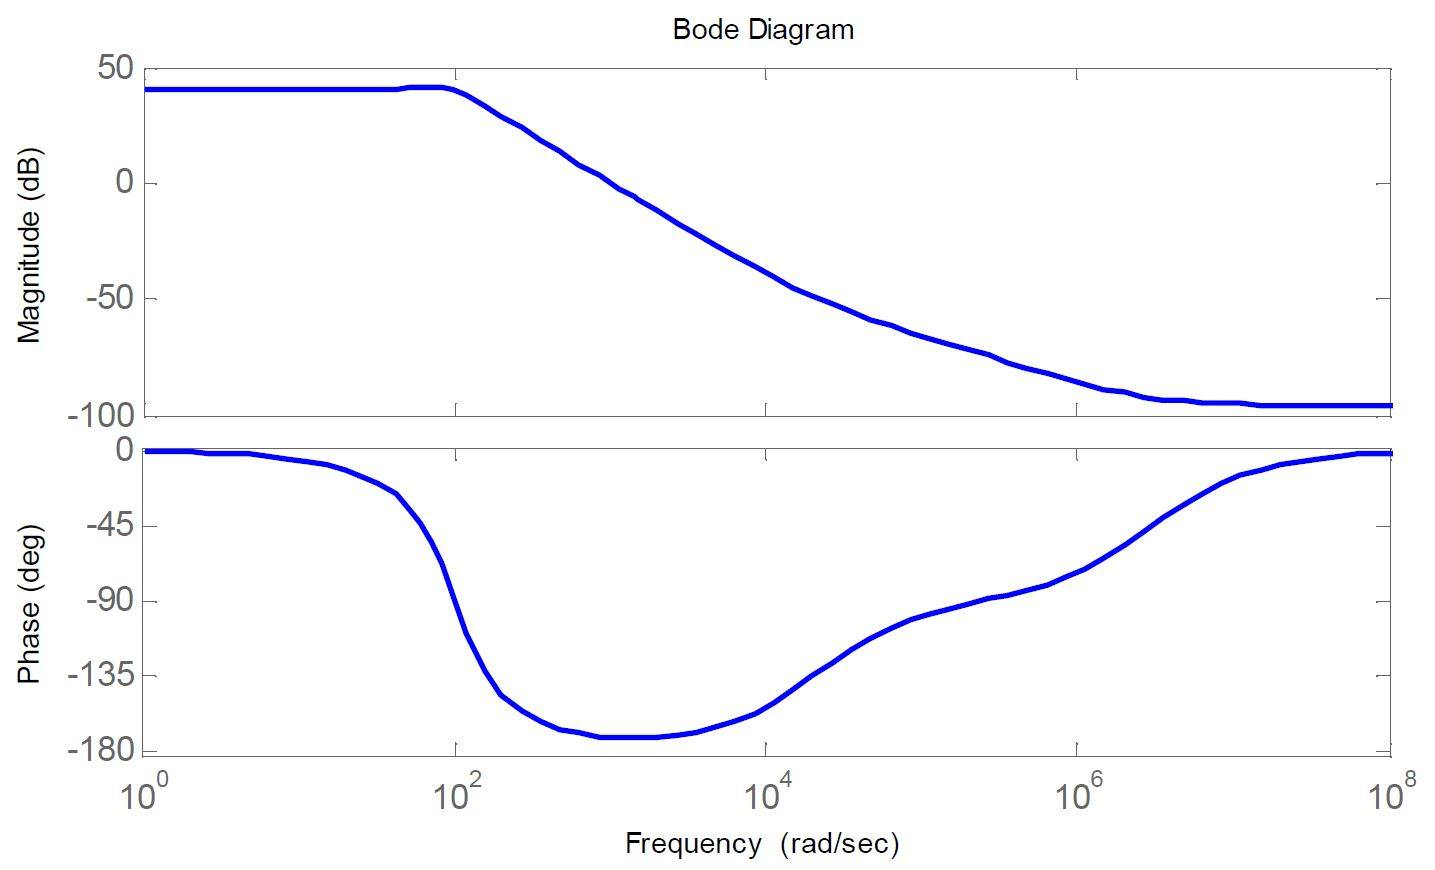
\includegraphics[width=12cm]{exo_bode}
\end{center}
Donnez la tension de sortie (sous forme temporelle) du système si la tension d’entrée est :
\begin{itemize}
\item $V_{in}(t)=1V\times cos(100\frac{rad}{s}t)$
\item $V_{in}(t)=5V\times cos(10^4\frac{rad}{s}t)$
\item $V_{in}(t)=2V\times cos(1000\frac{rad}{s}t+\frac{\pi}{6})$
\end{itemize}
}
{}

\newpage
\begin{center}
\begin{tikzpicture}
	\begin{loglogaxis}[
		xmin=1e-1, xmax=1e5,
		ymin=1e-1, ymax=1e5,
		yticklabels={,,},
		xticklabels={,,},
		grid=both,
		width=17cm,
		height=17cm,
		major grid style={black!50}
		]
	\end{loglogaxis}
\end{tikzpicture}
\end{center}

\begin{center}
\begin{tikzpicture}
	\begin{axis}[
		xmode=log,
		xmin=1e-1, xmax=1e5,
		ymin=1, ymax=9,
		yticklabels={,,},
		xticklabels={,,},
		grid=both,
		width=17cm,
		height=9cm,
		major grid style={black!50}
		]
	\end{axis}
\end{tikzpicture}
\end{center}

\newpage
\begin{center}
	\begin{center}
	\begin{tikzpicture}
		\begin{loglogaxis}[
			xmin=1e-1, xmax=1e5,
			ymin=1e-1, ymax=1e5,
			yticklabels={,,},
			xticklabels={,,},
			grid=both,
			width=17cm,
			height=17cm,
			major grid style={black!50}
			]
		\end{loglogaxis}
	\end{tikzpicture}
	\end{center}

	\begin{center}
	\begin{tikzpicture}
		\begin{axis}[
			xmode=log,
			xmin=1e-1, xmax=1e5,
			ymin=1, ymax=9,
			yticklabels={,,},
			xticklabels={,,},
			grid=both,
			width=17cm,
			height=9cm,
			major grid style={black!50}
			]
		\end{axis}
	\end{tikzpicture}
	\end{center}
\end{center}
\end{document}
